\section{System Overview}
\label{sec:overview}

\begin{figure}[t]
  \centering
  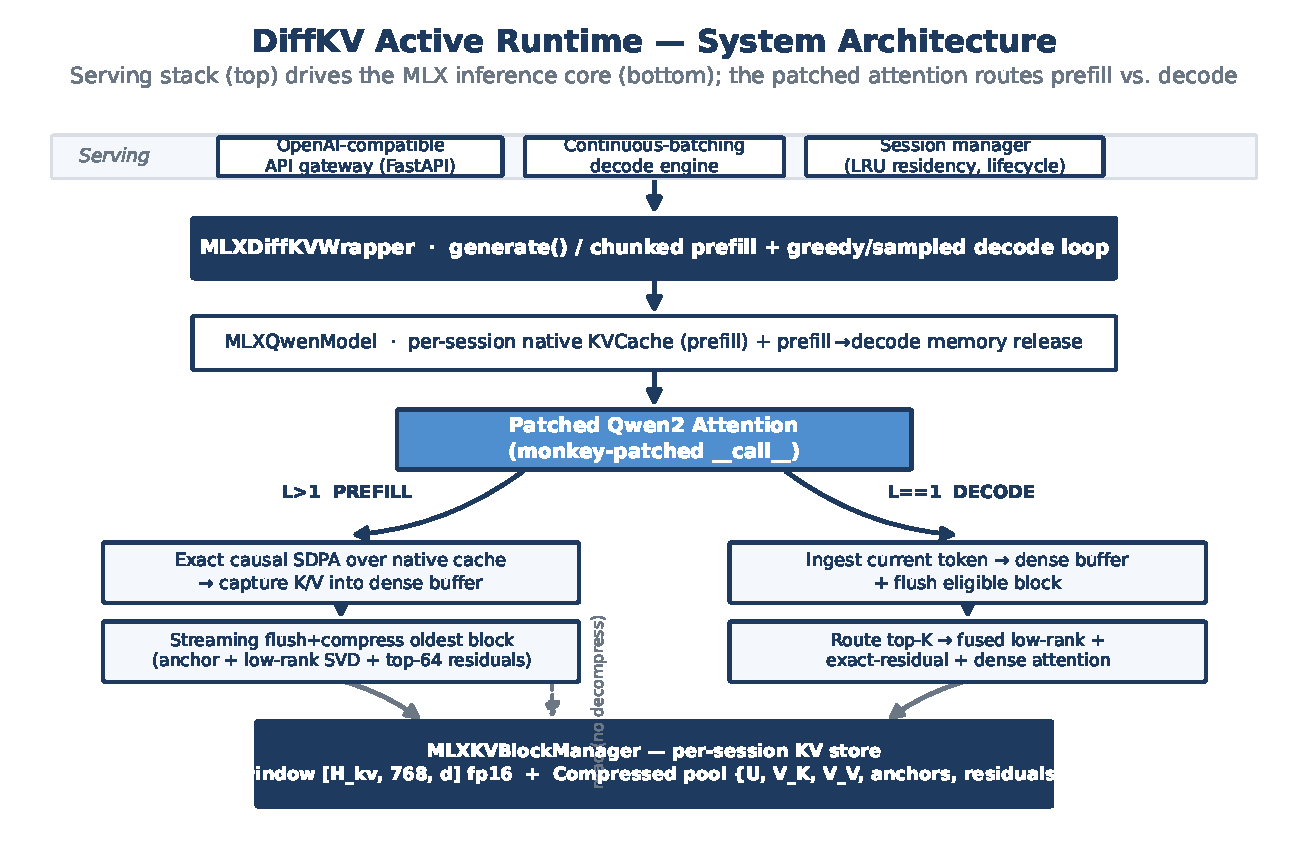
\includegraphics[width=\linewidth]{figures/f1_architecture.pdf}
  \caption{\diffkv{} active-runtime architecture. A serving stack (gateway, batching engine,
  session manager) drives \texttt{MLXDiffKVWrapper}, which runs chunked prefill and a greedy or
  sampled decode loop over \texttt{MLXQwenModel}. The model's attention layer is monkey-patched:
  on prefill ($L{>}1$) it runs (block-sparse) causal attention over the native cache and captures
  $K$/$V$ into the store; on decode ($L{=}1$) it ingests the current token and runs the fused
  routed sparse attention. All state lives in the per-session \texttt{MLXKVBlockManager}: a dense
  recency window plus a bounded compressed block pool.}
  \label{fig:arch}
\end{figure}

\diffkv{} is structured as a thin serving stack over an MLX inference core whose attention has
been replaced (Figure~\ref{fig:arch}). We walk the components in the order data flows through
them.

\paragraph{Serving.} An OpenAI-compatible gateway and a continuous-batching decode engine accept
requests; a session manager owns per-conversation lifecycle and residency. These layers are
standard and are not the subject of this paper; they exist so that the compression runtime is
exercised under a realistic request path.

\paragraph{Wrapper and model.} \texttt{MLXDiffKVWrapper} loads an \texttt{mlx\_lm} model, patches
its attention, and exposes \texttt{generate()}, which tokenizes the prompt, runs prefill in
fixed-size chunks, and then decodes one token at a time. \texttt{MLXQwenModel} wraps the patched
model, holds a native MLX KV cache used only during prefill, and---critically---\emph{releases}
that prefill cache at the prefill$\to$decode boundary so that decode-time memory reflects the
compressed store rather than a retained full-context cache (\S\ref{sec:runtime}).

\paragraph{Patched attention.} The heart of the system is a replacement for the model's attention
\texttt{\_\_call\_\_}. It branches on sequence length. During prefill ($L{>}1$) it computes causal
attention---optionally block-sparse (\S\ref{sec:runtime})---over the growing native cache to
produce correct hidden states, and captures each chunk's $K$/$V$ into the store. During decode
($L{=}1$) it ingests the newly generated token's $K$/$V$ into the dense window and computes the
attention output from the compressed store via the fused routed kernel (\S\ref{sec:decode}).

\paragraph{The store.} \texttt{MLXKVBlockManager} holds all persistent state, per session and per
layer: a \emph{dense recency window} of the most recent $\dwin{+}\bs{=}768$ tokens in exact fp16,
and a \emph{compressed block pool} of up to $M{=}256$ blocks, each holding the anchor, low-rank
factors, exact residuals, and router statistics for one $256$-token span. The pool is
pre-allocated and fixed in size, which is what bounds the runtime's memory
(\S\ref{sec:runtime}, Figure~\ref{fig:mem3d}).

\paragraph{Two data paths, one store.} Prefill \emph{fills} the store (capture, then stream-compress
the oldest blocks as the window overflows); decode \emph{reads} it (route, reconstruct in
low-rank space, attend residuals and window). The compression pipeline (\S\ref{sec:compression})
defines the store's contents; the runtime (\S\ref{sec:runtime}) defines its lifecycle; the decode
kernel (\S\ref{sec:decode}) defines how it is read. We take these in turn.

\paragraph{Scope.} This report documents the \emph{active runtime}---the MLX implementation.
An independent native (C++/GGML) engine and a CUDA/Triton decode kernel exist in the repository
and are out of scope here; we neither evaluate them nor compare against them, and where the
design ports cleanly we say so and reserve space for future measurement (\S\ref{sec:limits}).
A separate factual-store / semantic-retrieval subsystem is present but disabled by default and
is not part of the evaluated system.
